%IMAGEM GLOBALIAZÇÕES
\begin{center}
    \begin{figure}[h]
        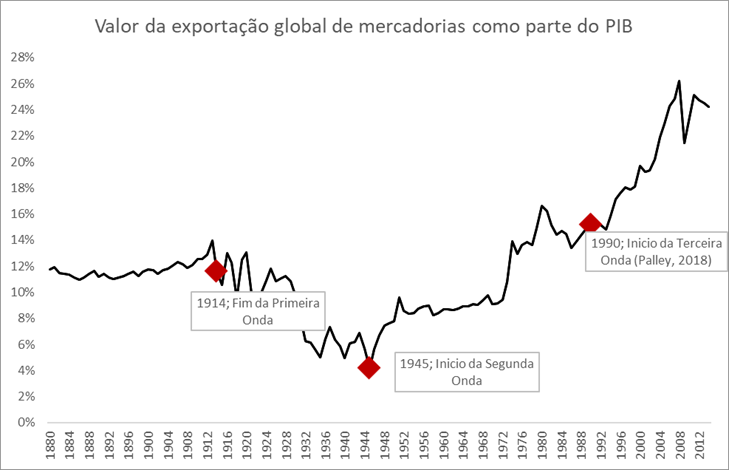
\includegraphics[width=0.8\textwidth]{globalização.png}
        \caption{Figura 1}
        \label{globalizacao}
    \end{figure}
\end{center}

%EXPORTAÇÃO RUSSIA
\begin{table}[h]
    \begin{center}
        \begin{tabular}{c}
            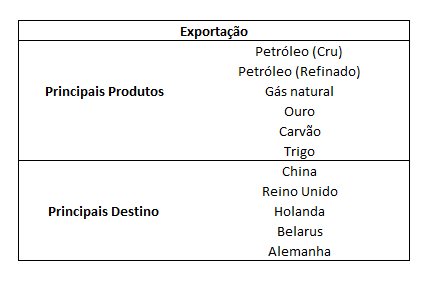
\includegraphics[width=0.8\textwidth]{exp rus.png}
        \end{tabular}
        \label{exprus}
        \caption{Tabela 1}
    \end{center}
\end{table}

%IMPORTAÇÃO RUSSIA
\begin{table}[h]
    \begin{center}
        \begin{tabular}{c}
            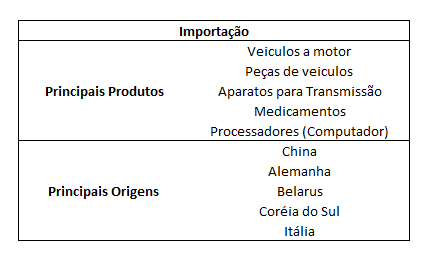
\includegraphics[width=0.8\textwidth]{imp rus.png}
        \end{tabular}
        \label{exprus}
        \caption{Tabela 1}
    \end{center}
\end{table}

%EXPORTAÇÃO UKRANIA
\begin{table}[h]
    \begin{center}
        \begin{tabular}{c}
            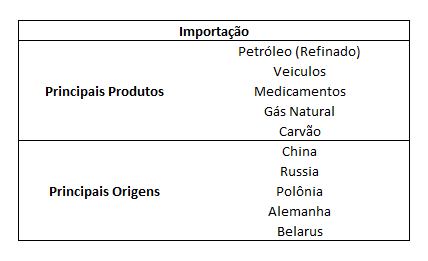
\includegraphics[width=0.8\textwidth]{imp ukr.png}
        \end{tabular}
        \label{exprus}
        \caption{Tabela 1}
    \end{center}
\end{table}

%IMPORTAÇÃO UKRANIA
\begin{table}[h]
    \begin{center}
        \begin{tabular}{c}
            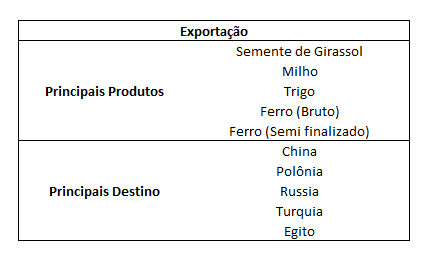
\includegraphics[width=0.8\textwidth]{exp ukr.png}
        \end{tabular}
        \label{exprus}
        \caption{Tabela 1}
    \end{center}
\end{table}

%BOXPLOT
\begin{figure}[h]
    \begin{center}
        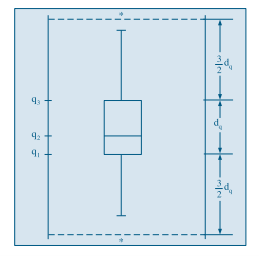
\includegraphics[width=0.8\textwidth]{boxplot.png}
        \caption{Figura 1}
        \label{globalizacao}
    \end{center}
\end{figure}

%REGRESSÃO LINEAR
$E(Y|x) = \mu (x) = \alpha + \beta x$

%Média aritmética
$\overline{x} = \frac{x_1 + ... + x_n}{n} = \frac{1}{n}\sum_{i = 1}^{n}  x_i$